%%%%%%%%%%%%%%%%%%%%%%%%%%%%%%%%%%%%%%%%%
% Beamer Presentation
% LaTeX Template
% Version 1.0 (10/11/12)
%
% This template has been downloaded from:
% http://www.LaTeXTemplates.com
%
% License:
% CC BY-NC-SA 3.0 (http://creativecommons.org/licenses/by-nc-sa/3.0/)
%
%%%%%%%%%%%%%%%%%%%%%%%%%%%%%%%%%%%%%%%%%

%----------------------------------------------------------------------------------------
%	PACKAGES AND THEMES
%----------------------------------------------------------------------------------------

\documentclass{beamer}

\mode<presentation> {

% The Beamer class comes with a number of default slide themes
% which change the colors and layouts of slides. Below this is a list
% of all the themes, uncomment each in turn to see what they look like.

%\usetheme{default}
%\usetheme{AnnArbor}
%\usetheme{Antibes}
%\usetheme{Bergen}
%\usetheme{Berkeley}
%\usetheme{Berlin}
%\usetheme{Boadilla}
%\usetheme{CambridgeUS}
%\usetheme{Copenhagen}
%\usetheme{Darmstadt}
%\usetheme{Dresden}
%\usetheme{Frankfurt}
%\usetheme{Goettingen}
%\usetheme{Hannover}
%\usetheme{Ilmenau}
%\usetheme{JuanLesPins}
%\usetheme{Luebeck}
\usetheme{Madrid}
%\usetheme{Malmoe}
%\usetheme{Marburg}
%\usetheme{Montpellier}
%\usetheme{PaloAlto}
%\usetheme{Pittsburgh}
%\usetheme{Rochester}
%\usetheme{Singapore}
%\usetheme{Szeged}
%\usetheme{Warsaw}

% As well as themes, the Beamer class has a number of color themes
% for any slide theme. Uncomment each of these in turn to see how it
% changes the colors of your current slide theme.

%\usecolortheme{albatross}
%\usecolortheme{beaver}
%\usecolortheme{beetle}
%\usecolortheme{crane}
%\usecolortheme{dolphin}
%\usecolortheme{dove}
%\usecolortheme{fly}
%\usecolortheme{lily}
%\usecolortheme{orchid}
%\usecolortheme{rose}
%\usecolortheme{seagull}
%\usecolortheme{seahorse}
%\usecolortheme{whale}
%\usecolortheme{wolverine}

%\setbeamertemplate{footline} % To remove the footer line in all slides uncomment this line
%\setbeamertemplate{footline}[page number] % To replace the footer line in all slides with a simple slide count uncomment this line

%\setbeamertemplate{navigation symbols}{} % To remove the navigation symbols from the bottom of all slides uncomment this line
}
\newcommand\tab[1][1cm]{\hspace*{#1}}
\usepackage{graphicx} % Allows including images
\usepackage{booktabs} % Allows the use of \toprule, \midrule and \bottomrule in tables

%----------------------------------------------------------------------------------------
%	TITLE PAGE
%----------------------------------------------------------------------------------------

\title[Analysis of 2APL]{Multi-Agent System Design:\\Analysis of the 2APL alanguage} % The short title appears at the bottom of every slide, the full title is only on the title page

\author[Aushev \and Medina \and Miralles \and Su\'arez]{Alex Aushev \and Salvador Medina \and Carles Miralles \and Alejandro Su\'arez} % Your name
\institute[UPC] % Your institution as it will appear on the bottom of every slide, may be shorthand to save space
{
Universitat Polit\`ecnica de Catalunya \\
}
\date{March 2017} % Date, can be changed to a custom date

\begin{document}

\begin{frame}
\titlepage % Print the title page as the first slide
\end{frame}

\begin{frame}
\frametitle{Overview} % Table of contents slide, comment this block out to remove it
\tableofcontents % Throughout your presentation, if you choose to use \section{} and \subsection{} commands, these will automatically be printed on this slide as an overview of your presentation
\end{frame}



%----------------------------------------------------------------------------------------
%	PRESENTATION SLIDES
%----------------------------------------------------------------------------------------

\section{Language Elements} 
\section{Multi-Agent transition rules}
\section{Execution of Multi-Agent System}
\section{Platform tools}
\section{Demo}
%------------------------------------------------
%\subsection{Subsection Example} % A subsection can be created just before a set of slides with a common theme to further break down your presentation into chunks


\begin{frame}
\frametitle{Introduction}
  \begin{itemize}
      \item BDI-based agent-oriented programming language.\\~\\
      
      \item Provides \textbf{programming constructions} to express the concepts in existing agent-oriented methodologies: \textit{Goals and Beliefs, Actions, Reasoning rules and Plans.}\\~\\
      
      \item Agent \textbf{deliberation cycle} to process agent constructions. \\~\\

      \item Has \textbf{formal semantics} that allows verify whether agent programs satisfy their specification.\\~\\
      \item Integrates \textbf{declarative and imperative} programming paradigms.\\~\\
      % TODO: something else?
  \end{itemize}
\end{frame}

%------------------------------------------------
\begin{frame}
\Huge{\centerline{Beliefs and Goals}}
\end{frame}
%------------------------------------------------
\begin{frame}
\frametitle{Beliefs}
\begin{block}{Definition}
	Information available to agent, expressed as facts and rules in Prolog. All facts are assumed to be ground.
\end{block}
\begin{block}{Syntax}
  Beliefs: \\ 
  \tab  pos(1,1).\\
  \tab hasGold(0).\\
  \tab trash(2,3).\\
  \tab clean(blockworld) :- not trash(\_,\_).
\end{block}
\end{frame}

%------------------------------------------------
\begin{frame}
\frametitle{Goals}
\begin{block}{Definition}
	List of logical formulas, each of which denoting a task the agent wants to accomplish (not necessary all at once).
\end{block}
\begin{block}{Syntax}
  Goals: \\
  \tab  hasGold(5) and clean(blockworld), hasGold(10) \\~\\
  (G1) agent gets 5 units of gold and the blockworld is clean \\ 
  (G2) the agent gets 10 units of gold (regardless the blockworld state)
\end{block}
\end{frame}

%------------------------------------------------
\begin{frame}
\Huge{\centerline{Actions}}
\end{frame}

%------------------------------------------------
\begin{frame}
\frametitle{Actions (I)}
	\begin{itemize}
    	\item \textbf{Capabilities} of an agent \\~\\
        \item \textbf{Passive} entities, \textbf{activated} in reasoning rules and plans\\~\\
        \item There are 5 kinds of:\\~\\
        \begin{itemize}
        	\item Update beliefs\\~\\
            \item Goals management \\~\\
            \item Agent communication\\~\\
            \item Environment interaction\\~\\
            \item Beliefs and Goals queries
        \end{itemize}
    \end{itemize}
\end{frame}
%------------------------------------------------
\begin{frame}
\frametitle{Actions (II)}
	\begin{block}{Update beliefs: \{Pre\} Action \{Post\}}
      BeliefUpdates:\\
        \tab \{not carry(gold)\} \textbf{PickUp()} \{carry(gold)\}\\
        \tab \{trash(X,Y) and pos(X,Y)\} \textbf{RemoveTrash()} \{not trash(X,Y)\}
    \end{block}
    
    \begin{block}{Goals dynamics: adopt/drop}
      adopta($\phi$), adoptz($\phi$) : Add the goal $\phi$ at the begining/end.\\~\\
      dropgoal($\phi$), dropsubgoal($\phi$), dropsupergoal($\phi$): drop goal $\phi$, all subgoals of $\phi$ and all supergoals of $\phi$.
  	\end{block}
    
    \begin{block}{Agent communication: send}
    	send(Receiver,Performative, Language,Ontology,Content)\\
        
        send(Receiver,Performative,Content). Simplified when is assumed a Language \& Ontology between agents.
	\end{block}
\end{frame}
%------------------------------------------------
\begin{frame}
\frametitle{Actions (III)}
   \begin{block}{Environment interaction: @env(ActionName,Return)}
    	env: Java class.\\
        ActionName: method that modifies the environment.\\
        Return: List of result values or empty list\\~\\
    	
        @blockworld(east(),L): go one step east in the blockworld environment.
	\end{block}
    
	\begin{block}{Test beliefs and goals: B()/G()}
      To check whether an agent has a belief/goal. \\	
      Beliefs:\tab p(a)\\
      Goals:\tab q(b)\\~\\
      B(p(X)) \& G(q(X)) \textbf{Fails} (not unifier), block the execution of the plan\\
      B(p(X) \& G(q(Y)) \textbf{Success} \{X/a, Y/b\}, instantiate variables in subsequent actions in the plan. 
	\end{block}
\end{frame}

%------------------------------------------------
\begin{frame}
\Huge{\centerline{Plans and Reasoning Rules}}
\end{frame}

%------------------------------------------------
\begin{frame}
\frametitle{Plans}
	\begin{itemize}
    	\item \textbf{Imperative} constructions to achieve the goals of an agent \\~\\
    	\item Sequence of actions composed by sequence/conditional/loop operator \\~\\
        \item Initial plan: how to start\\~\\
        \item Goal Plans: How to achieve goals\\~\\
        \item Recovery Plans: backup plans\\~\\
        \item Procedure Plans: plans for external events or input messages or abstract actions\\~\\
	\end{itemize}
\end{frame}

%------------------------------------------------
\begin{frame}
\frametitle{Plans}
	\begin{block}{Initial Plan}
      Plans:\\
      \tab $[@blockworld(enter(5,5,red),L);ChPos(5,5) ]$\\
      \tab $send(admin,request,register(me))$\\~\\
    Updates my beliefs base with initial position 5,5 after entering into the blockworld ($[]$Atomic). \\
    Request the administrator to register him.
    \end{block}
\end{frame}
%------------------------------------------------
\begin{frame}
\frametitle{Planning goal rules (PG-Rules)}
	\begin{block}{Syntax}
    	$[<goalquery>]\leftarrow\ <belquery> | <plan> $ \\
        \begin{itemize}
    	\item Generates a plan if agent has goals in goalquery and fulfill belief conditions.
    	\item Goal is optional which means that a plan can be generated only based on beliefs conditions.
        \end{itemize}
    \end{block}
    
    \begin{block}{Example}
    	PG-Rules:\\
        \tab $clean(R)\leftarrow \ pos(X1,Y1)\ and\ trash(X2,Y2)\ |$ 
        \tab \tab $\left\{[goto(X1,Y1,X2,Y2); RemoveTrash()]\right\} $ \\
        \begin{itemize}
        	\item If agent has the clean goal it beliefs that there are trash in X2,Y2 then a plan is generated for going from X1,Y1 to X2,Y2 and remove the trash
        	\item goto() is an abstract action (next section)
        \end{itemize}
	\end{block}
    
\end{frame}

%------------------------------------------------
\begin{frame}
\frametitle{Procedure call Rules (PC-Rules)}
	\begin{block}{Definition}
    	It allows generate plans as response to:
        \begin{itemize}
            \item \textbf{messages} sent by other agents 
            \item \textbf{events} generated by external environment 
            \item \textbf{the execution} of abstract actions
        \end{itemize}
    \end{block}
    
    \begin{block}{Example}
    	PC-rules:\\
  		\tab message(A,inform,La,On,goldAt(X2,Y2)) $\leftarrow$  not carry(gold) $|$\\
        \tab \tab \tab \{ getAndStoreGold(X2,Y2) \}\\
        \tab event(gold(X2,Y2),blockworld) $\leftarrow$  not carry(gold) $|$\\
    	\tab \tab \tab \{ getAndStoreGold(X2,Y2) \}\\ 
        \tab getAndStoreGold(X,Y) $\leftarrow$ pos(X1,Y1) $|$ \{ \\
    	\tab \tab  $[$ goTo(X1,Y1,X,Y);@blockworld(pickup(),\_); PickUp(); \\
        \tab \tab  goTo(X,Y,s3,s3);@blockworld(drop(),\_);StoreGold() $]$ \} 
    \end{block}
\end{frame}
%------------------------------------------------
\begin{frame}
\frametitle{Plan repair Rules (PR-Rules)}
  \begin{block}{Definition}
	$<plan>\leftarrow\ <belquery> | <plan> $ \\~\\
    A plan fails if:
   	\begin{itemize}
   	 	\item The precondition of a belief update action is not entailed by the belief base
   	 	\item If there is not applicable procedure rule for an abstract action
        \item If an external actions throws an ExternalActionFailedException
        \item The agent doesn't have access to an external environment 
        \item An external action is not defined for an environment
        \item A test expression is not entailed by the belief and goal bases
        \item A goal being adopted that is already in the belief base or the goal is not ground
        \item An atomic plan if one action of the plan fails
   	\end{itemize} 
  \end{block}
\end{frame}

%------------------------------------------------
\begin{frame}
\frametitle{Plan repair Rules (PR-Rules)}
	\begin{block}{Example}
		PR-Rules:\\
        \tab $@blockworld(east(),\_);@blockworld(east(),\_);X \leftarrow true | $\\
	    \tab \tab $\{ @blockworld(north(),_);@blockworld(east(),_);$ \\
         \tab \tab $@blockworld(east(),_);@blockworld(south(),_);X \}$ \\~\\
         
	A \textbf{failing plan} starting with $@blockworld(east(),\_);@blockworld(east(),\_);$ generates this repair plan (X is whatever other action)
    \end{block}
\end{frame}

% -----------------------------------------------

\begin{frame}
\frametitle{External environments}
\begin{itemize}
	\item We would like to interact and get feedback from the environment
	\item Agents can interact with external environments (or vice-versa) via:
    \begin{itemize}
    	\item External actions
        \item External events
        \item Exceptions
    \end{itemize}
\end{itemize}
\end{frame}

%------------------------------------------------
\begin{frame}
\Huge{\centerline{2APL Semantics}}
\end{frame}

%------------------------------------------------

\begin{frame}
\frametitle{2APL Configuration (I)}

\begin{block}{ Individual Agent}
The configuration of an individual 2APL agent is defied as $ A_\iota = \{\iota, \sigma, \gamma , \pi, \theta, \epsilon \} $.
\end{block}
Where:
\begin{itemize}
\item $\iota$ is the Agent's Identifier
\item $\sigma$ is a set of belief expressions
\item $\gamma$ is a list of goal expressions
\item $\pi$ is a set of plans in $(\pi, r, p)$ where $\pi$ is the plan, $r$ are the PG\_rules and $p$ is the identifier
\item $\theta$ is a ground substitution (binds variables)
\item $\epsilon = E,I,M$ where $E$,$I$ and $M$ are external events, failed plans and messages respectively
\end{itemize}

\end{frame}

\begin{frame}
\frametitle{2APL Configuration (II)}

\begin{block}{ Individual Agent}
The configuration of a 2APL multi-agents system is defined as $\{A_1,...,A_n, \chi\}$.
\end{block}
Where:
\begin{itemize}
\item $A_i$ is the configuration of Agent i
\item $\chi$ is a set of external shared environments
\item In the initial state, $\theta=\emptyset$ and $\epsilon=\{\emptyset,\emptyset,\emptyset\}$ for all agents
\item The configuration is updated at each iteration by means of the transition rules
\end{itemize}

\end{frame}

%------------------------------------------------
\begin{frame}
\Huge{\centerline{Multi-Agent transition rules}}
\end{frame}

%------------------------------------------------

\begin{frame}
\frametitle{Multi-Agent transition rules (I)}

\begin{block}{Basic Actions}
	$\frac{A_i \rightarrow A^{\prime}_i}{\{A_1,...,A_i,..,A_n,\chi\} \rightarrow \{A_1,...,A^{\prime}_i,..,A_n,\chi\}}$, this is, basic actions of agent $i$ do not affect the environment nor other agents 
\end{block}

\begin{block}{External Actions (I)}
	$\frac{F^{env}_{\iota,\alpha}(t_1,...,t_n,\chi) = (t, \chi^\prime)}{ \chi \xrightarrow[]{env(\iota,\alpha(t_1,...,t_n),t)} \chi^\prime}$, this is, when an external action is broadcasted, the environment can make a transition according to it
\end{block}

\begin{block}{External Actions (II)}
	$\frac{ A_i \xrightarrow[]{env(\iota,\alpha(t_1,...,t_n),t)} A^\prime_i \&\& \chi \xrightarrow[]{env(\iota,\alpha(t_1,...,t_n),t)} \chi^\prime}{\{A_1,...,A_i,..,A_n,\chi\} \rightarrow \{A_1,...,A^{\prime}_i,..,A_n,\chi^\prime\} }$, this is, if a external action by agent $A_i$ changes the environment, it can be the only one noticing it
\end{block}

\end{frame}

%------------------------------------------------

\begin{frame}
\frametitle{Multi-Agent transition rules (II)}

\begin{block}{Internal environment dynamics}
	$\frac{ env \in \chi \& env \xrightarrow{(\theta,(k,...,l))!} env^\prime}{\{A_1,...,A_i,..,A_n,\chi\} \rightarrow \{A^\prime_1,...,A^{\prime}_i,..,A^\prime_n,\chi^\prime\} }$, this is, which agents receives an event is the decision of the environment designer
\end{block}

\begin{block}{Message passing}
 $ \frac{A_i \xrightarrow[]{\varphi!} A^\prime_i \& A_j \xrightarrow[]{\varphi?} A^\prime_j}{\{A_1,...,A_i,A_j,...,A_n,\chi\} \rightarrow \{A^\prime_1,...,A^{\prime}_i,A^\prime_j,...,A^\prime_n,\chi^\prime\} } $, this is, when an agent sends a message to another agent, both transitions (send and receive) are done synchronously
\end{block}

\end{frame}

%------------------------------------------------

% Executing MAS section
%%------------------------------------------------
\begin{frame}
\Huge{\centerline{Execution of Multi-Agent Systems}}
\end{frame}

%------------------------------------------------

\begin{frame}
\frametitle{Semantics of Computational Run }
\begin{block}{Definition}
	The execution of a 2APL multi-agent system with initial configuration $A_1,...,A_n, χ$ is the set of computation runs $CR(A_1,...,A_n, χ)$ of the 2APL transition system.
\end{block}


\begin{block}{Definition}
	A computation run $CR(s0)$ is a sequence $s_0,...$ where $s_i$ is a
configuration, and $∀i>0 : s_i−1 → s_i$ is a transition in the transition system.
\end{block}

\end{frame}


%------------------------------------------------

\begin{frame}
	\frametitle{Single-Agent Deliberation Cycle}
    \begin{figure}
      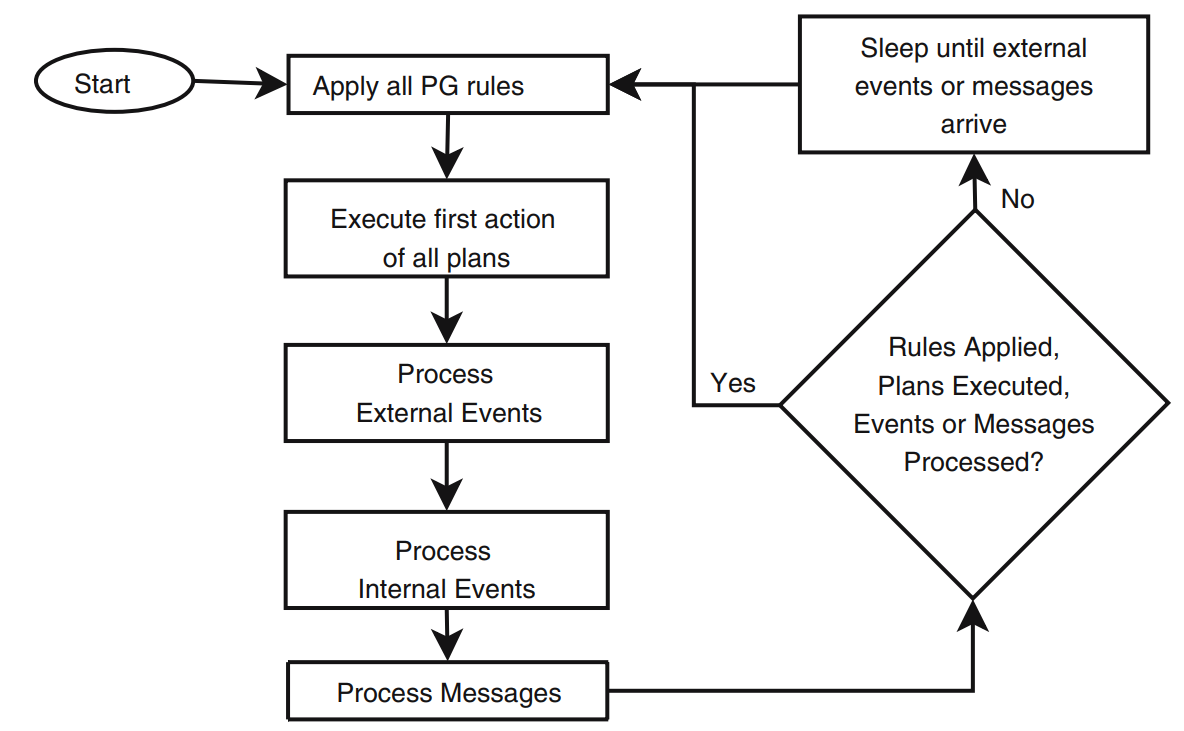
\includegraphics[width=1\textwidth]{deliberation-cycle-individual-2apl}}
    \end{figure}
\end{frame}

%------------------------------------------------

\begin{frame}
\Huge{\centerline{Execution of Multi-Agent Systems}}
\end{frame}

%------------------------------------------------

\begin{frame}
\frametitle{Semantics of Computational Run }
\begin{block}{Definition}
	The execution of a 2APL multi-agent system with initial configuration $A_1,...,A_n, \chi$ is the set of computation runs $CR(A_1,...,A_n, \chi)$ of the 2APL transition system.
\end{block}
\begin{block}{Definition}
	A computation run $CR(s0)$ is a sequence $s_0,...$ where $s_i$ is a
configuration, and $ \forall{i>0} : s_{i−1} \rightarrow s_i$ is a transition in the transition system.
\end{block}

\end{frame}


%------------------------------------------------

\begin{frame}
	\frametitle{Single-Agent Deliberation Cycle}
    \begin{figure}
      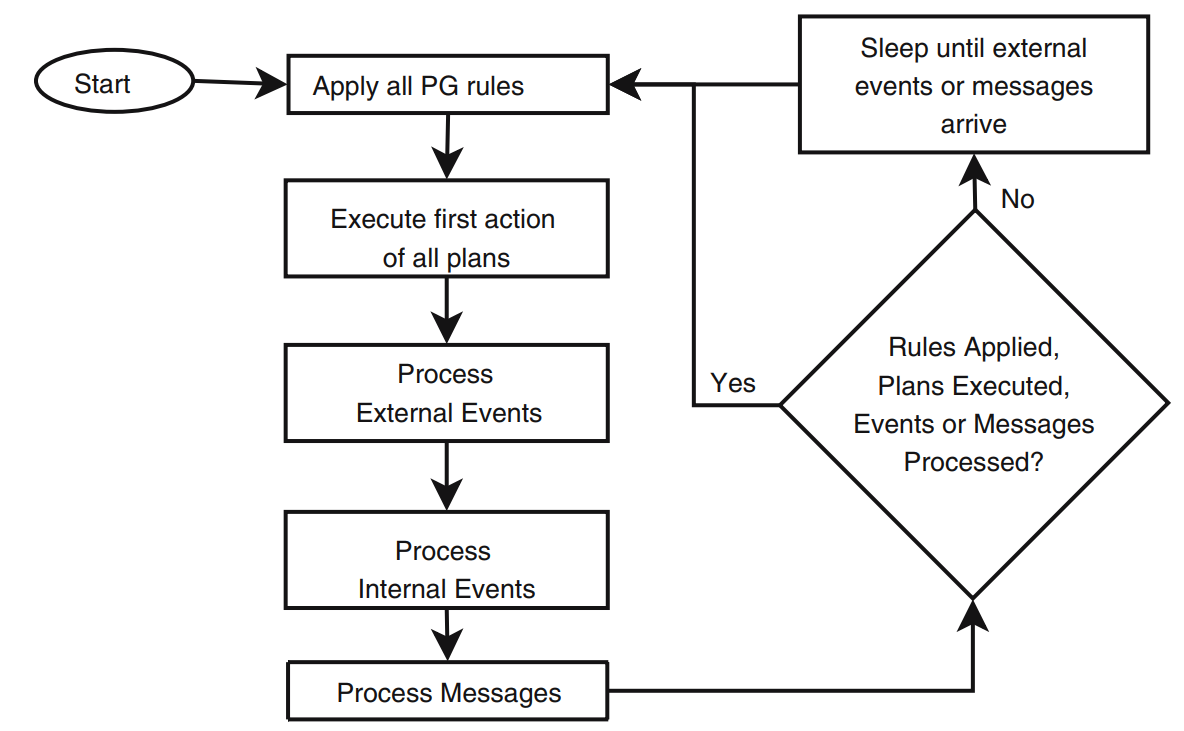
\includegraphics[width=1\textwidth]{deliberation-cycle-individual-2apl}
    \end{figure}
\end{frame}

%------------------------------------------------

\begin{frame}
\frametitle{Characteristics of the Deliberation Cycle (I)}
  \begin{itemize}
  
      \item The interpreter of 2APL executes individual agents and the environment in
parallel in an interleaving mode.\\~\\
      
      \item Each cycle starts by applying all applicable PG-rules, each rule only one time. \\~\\
      
      \item The DC proceeds by executing only the first actions of all plans. In order to allow all plans to get a chance to be executed. \\~\\
      
      \item  Internal and external events and messages are processed by applying the first applicable PC-rule. \\~\\
      
  \end{itemize}
\end{frame}

\begin{frame}
\frametitle{Characteristics of the Deliberation Cycle (II)}
  \begin{itemize}
  
     \item If the execution of a plan fails, then the plan will either be repaired in the same
deliberation cycle or get re-executed in the next deliberation cycle. \\~\\

	\item If the first action of a failed plan is a belief update, test, adopt
goal, abstract or external action and there is no plan repair rule to
repair it, then the failed plan may be successfully executed in the next deliberation cycle. \\~\\

  \end{itemize}
\end{frame}


% ----------------------------------------------------------

\begin{frame}
\Huge{\centerline{2APL platform}}
\end{frame}

\begin{frame}
\frametitle{Requirements}
	\begin{itemize}
	\item OS: Windows, Mac OS X, Linux and Unix (Solaris);
    \item Java Runtime Environment (JRE) 6 or Java Developers Kit (JDK) 6;
    \item 2APL website URL: http://apapl.sourceforge.net/
	\end{itemize}
    
	\begin{figure}
	
\includegraphics[width=0.9\linewidth]{images/2APLdownload.png}
    \caption{Download options for the platform on the 2APL website}
	\end{figure}
\end{frame}


\begin{frame}
\frametitle{How to run the platform}
2apl.jar can be run in two ways:
	\begin{itemize}
	\item directly (from the command line or windows interface);
    \item as a module for Eclipse;
	\end{itemize}

The platform allows communication among agents and can run on several machines connected in a network (on top of the Jade platform);

    \begin{figure}
	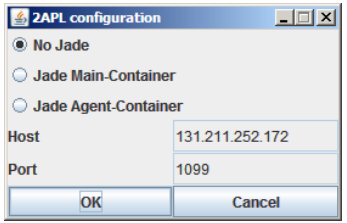
\includegraphics[width=0.4\linewidth]{images/2APLconf.png}
    \caption{2APL configuration options}
	\end{figure}
  
\end{frame}

\begin{frame}
\frametitle{2APL project components}
	\begin{itemize}
	\item  The MAS specification file. This is a text file with the extension .mas that contains an XML specification of the multiagent system. The name and path to the source of all agents and environments that start in the application are denoted here.
    \item A 2APL agent file. This is a text file with the extension .2apl and contains the 2APL code of the agent.
    \item An environment file. This is a runnable JAR (with the extension .jar)
	\end{itemize}
\end{frame}


\begin{frame}
\frametitle{2APL Platform}

    \begin{figure}
	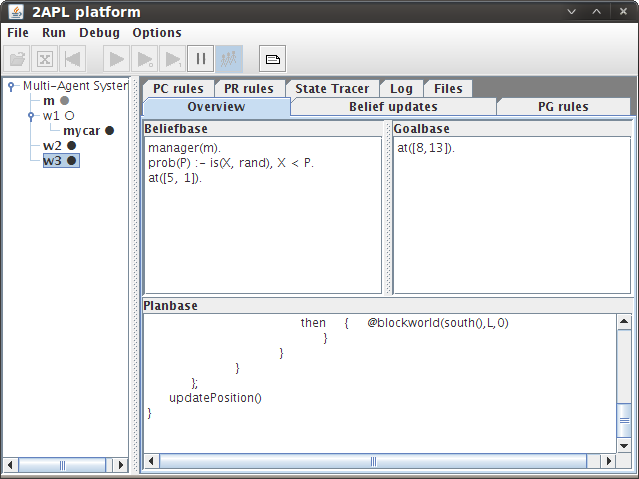
\includegraphics[width=0.75\linewidth]{images/2APLplatform.png}
    \caption{2APL platform interface}
	\end{figure}
  
\end{frame}

\begin{frame}
\frametitle{Eclipse plug-in}
	\begin{figure}
	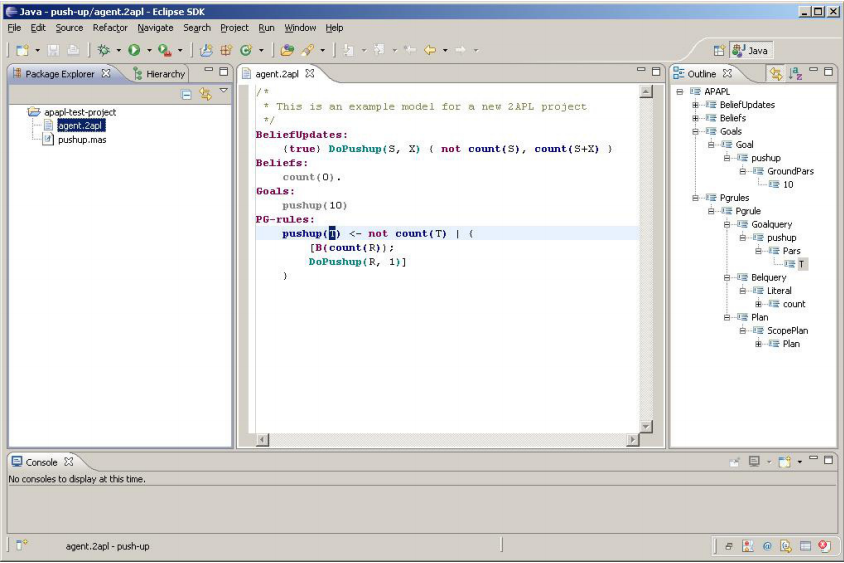
\includegraphics[width=0.85\linewidth]{images/2APLeclipse.png}
    \caption{2APL platform in Eclipse}
	\end{figure}
\end{frame}


\begin{frame}
\frametitle{Additional Tools}
	\begin{block}{Monitoring Tools}
	\begin{itemize}
   	\item Auto-update Overview tool;
    \item The State Tracer;
	\item Log tool.
    \end{itemize} 
	\end{block}
    
    These tools can be deactivated to improve the execution performance of the 2APL platform. The activation of the tools generates specific information and presents them in the corresponding tabs. 
	
\end{frame}

\begin{frame}
\frametitle{Auto-update Overview tool}
When this tab is active, the beliefs, goals, and plans of the current state of the selected agent are presented in the Beliefbase, Goalbase, and Planbase panels, respectively.

	\begin{figure}
	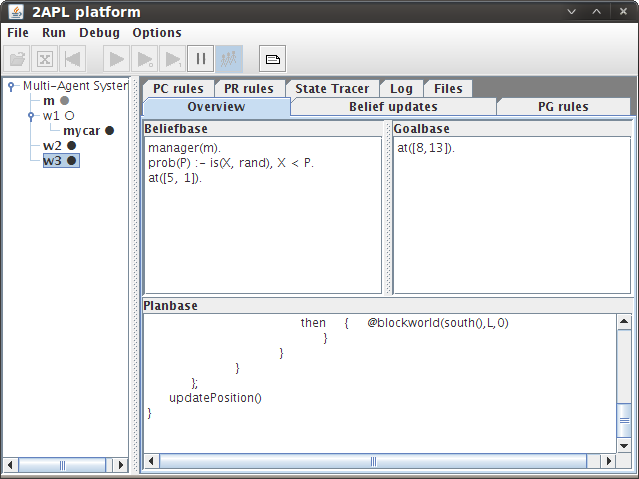
\includegraphics[width=0.65\linewidth]{images/2APLplatform.png}
	\end{figure}
\end{frame}

\begin{frame}
\frametitle{State Tracer}
Stores the beliefs, goals, and plans of all agents during execution. This tool allows a user to execute a multi-agent program for a while, pause the execution, and browse through the execution of each agent.

	\begin{figure}
	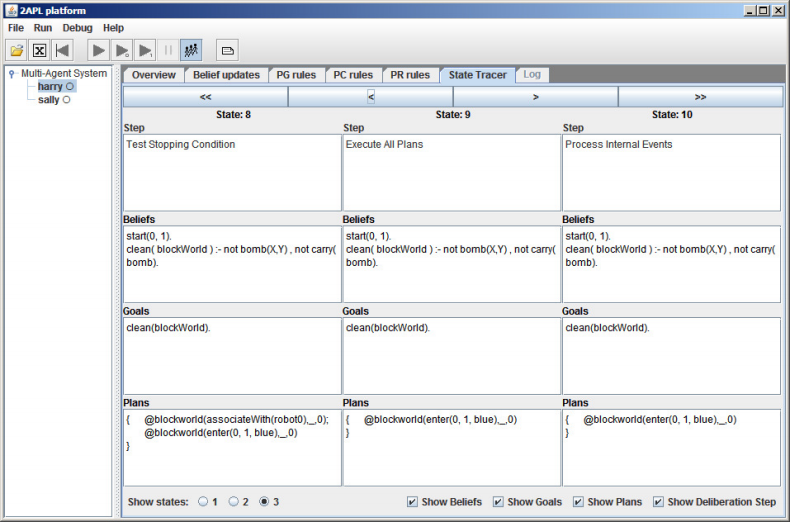
\includegraphics[width=0.65\linewidth]{images/2APLStateTracer.png}
	\end{figure}
\end{frame}

\begin{frame}
\frametitle{Log tool}
Presents information about the deliberation steps of individual agents. The user can browse through this window to see which deliberation steps have been preformed.

	\begin{figure}
	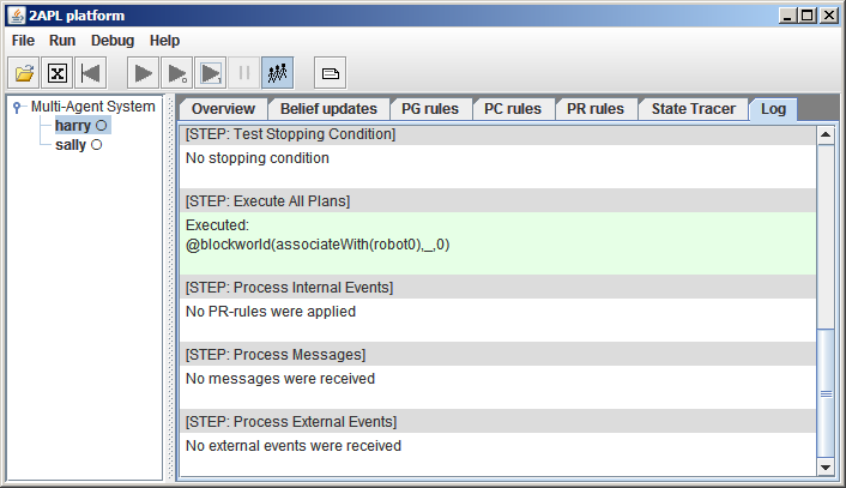
\includegraphics[width=0.65\linewidth]{images/2APLLog.png}
	\end{figure}
\end{frame}

\begin{frame}
\frametitle{Summary of platform features}
Programming Constructs
	\begin{itemize}
	\item \textbf{Multi-Agent System} Which and how many agents to create? Which environments? Which agent can access which environment?
	\item \textbf{Individual Agent} Beliefs, Goals, Plans, Events, Messages.
	\end{itemize}
    
Programming Principles and Techniques
	\begin{itemize}
	\item \textbf{Abstraction} Procedures and Recursion in Plans;
	\item \textbf{Error Handling} Plan Failure and their revision by Internal Events, Execution of Critical Region of Plans;
	\item \textbf{Legacy Systems} Environment and External Actions;
    \item \textbf{Encapsulation} Including 2APL files in other 2APL files;
    \item \textbf{Autonomy} Adjustable Deliberation Process.
	\end{itemize}

\end{frame}

%\begin{frame}
%\Huge{\centerline{Connecting with other alternatives}}
%\end{frame}

%\begin{frame}
%\frametitle{Semantic difference: 2APL vs 3APL}
%\end{frame}

%\begin{frame}
%\frametitle{Semantic difference: 2APL vs Jason}
%\end{frame}

%------------------------------------------------

\begin{frame}
\frametitle{References}
\footnotesize{
\begin{thebibliography}{99} % Beamer does not support BibTeX so references must be inserted manually as below
\bibitem[Smith, 2012]{p1} John Smith (2012)
\newblock Title of the publication
\newblock \emph{Journal Name} 12(3), 45 -- 678.
\end{thebibliography}
}
\end{frame}

%------------------------------------------------

\begin{frame}
\Huge{\centerline{The End}}
\end{frame}

% ----------------------------------------------------------------------------------------

\end{document}